\documentclass[fleqn,10pt]{wlscirep}
\usepackage[utf8]{inputenc}
\usepackage[T1]{fontenc}
\usepackage{booktabs}
\usepackage{float}

\title{Game Store Price Recommendation and Summarization}

\author[1,*]{Muhammed Pašić}
\author[1,+]{Armin Memišević}
\affil[1]{Data Engineering and Machine Learning Project, supervised by Prof.\ Aida Brankovi\'{c}}

\affil[*]{Data Engineering (CDA) lead: database design, API/data acquisition, cleaning, fuzzy matching, price summarization}

\affil[+]{Machine Learning (MLPR) lead: feature engineering, k-Nearest Neighbour recommender, evaluation, Streamlit application}

\begin{abstract}
The following report outlines a platform that merges game meta information collected from the RAWG API with game prices recorded on the Steam and Epic Games Store websites, resolves the two with approximate string matching, and creates recommendations with a content-based k-Nearest Neighbours classifier. The functionality can be accessed through a three-page Streamlit app. Out of 3,000 games collected from the RAWG API, 915 games from the Epic Games Store and 988 from the Steam store have been loaded. TheFuzz token-sort matching resolved 446 of the 915 Epic Games games (48.7\%), and 287 of the 988 Steam games (29.0\%) at a confidence threshold of 80\%, which results in a list of 508 games with at least one known store price. Both Streamlit app and recommender need a confirmation of prices on both the Epic Games and Steam (HAVING COUNT(DISTINCT store) = 2) before comparing and recommending any game. The direct verification against the delivered database reveals that only 21 of the 3,000 games in our catalog currently meet such requirement. Thus, the strict filtering criterion ensures the completeness of the price comparison at the expense of catalog coverage, which has been determined to be the core, honest finding of this report.
Furthermore, the following four components have been found to work and verified directly in the delivered code: a cache-enabled autocomplete search bar with game names that are already validated for both stores; an in-app “Admin \& ML Metrics” dashboard that runs the recommender evaluation script as a subprocess, outputs Precision@5, Recall@5, and F1@5 metrics (which currently stand at 0.0371, 0.0485, and 0.0420 respectively at the time of writing), and shows the precision-recall graph; a standalone audit queue script that exports all unresolved price rows into a CSV file for human verification; and a price summarization script that produces the price comparison between the two stores as outlined in the original project brief.
Exploratory data analysis of Metacritic score distribution, genre popularity and cross-store price distribution is done in the report before feature scaling and encoding used in the recommender are justified.
\end{abstract}

\begin{document}

\flushbottom
\maketitle
\thispagestyle{empty}

\section*{Introduction}

The online digital game storefronts (Steam, Epic Games Store, GOG, etc.) represent independent, closed catalogs. The same game is listed with different names, versions, and prices, and none of them has a canonical identifier that would make the record merging process for a third party automated. An individual who wants to buy the cheapest copy of the game in question or to be recommended new games based on the titles owned needs to do it manually by comparing several web pages of different stores. This problem in its essence is what the project is intended to solve: (i) collecting official data about games and pricing of the store in one database; (ii) unifying the heterogeneous list of titles represented by each store separately (e.g., "The Witcher 3: Wild Hunt -- Complete Edition" vs. "The Witcher 3: Wild Hunt") to one internal identifier of the game; (iii) creating an actual cross-store comparison using the aforementioned price records; and (iv) suggesting new games to the user based on the games the user already likes, without having to interact with the system before (cold-start problem) \cite{Zhang:coldstart:2025}.

Two domain factors affect every subsequent decision in this project. Firstly, metadata for games (titles, genres, dates of release, critic scores) and game pricing are separate concepts, both logically and practically: metadata modifications happen rarely and can be handled easily with the help of an aggregate API (RAWG) while prices constantly change and come directly from stores. That resulted in creating a schema with two tables (Games and Prices) rather than a single denormalized one. Secondly, entity resolution across catalogs has its probabilistic nature due to the absence of a common key and the necessity to match games' titles based on fuzzy string similarity; this match provides confidence estimation only. Thus, the \texttt{match\_confidence} numeric field is included on every row in the Prices table instead of choosing the highest-scoring match automatically.

Every number and figure shown below is directly extracted from the \texttt{game\_platform.db} and related source files to provide an accurate representation of the real state of the project as opposed to the intended design.

\section*{Methods}

\subsection*{Data sources and schema}

There are three datasets to be used as input. (1) RAWG API\cite{RAWG:api}: 3,000 games were fetched in order of popularity (-added), retaining title, release date, genres, developer, Metacritic score and cover picture and added to a Games table using the RAWG game ID as key. (2) Epic Games Store: As Epic doesn't provide any public pricing API and their store is implemented as a JavaScript single-page application, the prices have to be fetched from a static CSV file (games.csv\cite{Kaggle:epicgamesstore}, 915 rows). (3) Steam: Pricing is fetched from two official endpoints, IStoreService/GetAppList (full app catalog) and store.steampowered.com/api/appdetails (\texttt{price\_overview} per app) \cite{Valve:webapi}. Valve has a rate limit on the second endpoint of about 200 requests every five minutes per IP address. This request in the \texttt{fetch\_steam\_prices.py} script is protected with an instance of check on the JSON response, as sometimes Steam replies with a list instead of an object for deleted or geographically restricted apps, which would otherwise cause an error in the loader. In addition, the loader limits the number of candidate titles to process through the --limit argument (100 by default) instead of loading all candidates in one go. There are three tables in the database schema (schema.sql): Games (metadata, RAWG ID as key), Prices (one row per listing, \texttt{game\_id}set NULL until mapping, \texttt{match\_confidence} filled after fuzzy matching) and \texttt{User\_Likes} (session-scoped likes for Streamlit interface).

\subsection*{Data preparation and cleaning}

The price variable in the Epic Games CSV is stored as an integer in cents; the \texttt{fix\_prices.py} script divides any price above 100 dollars by 100. While this solution works for the observed catalog, it is not a currency-unit normalization and fails for more expensive items with a price of over 100 dollars. The inconsistency between Steam and Epic prices is manifested through their different approaches to marking games that are either free-to-play or whose price cannot be determined – Steam returns None from its \texttt{fetch\_price\_for\_app} method and omits such apps from its output completely, while Epic marks free titles by assigning them a price value of 0.00 dollars (73 instances, 8.0\% of Epic Games). Thus, the final output Prices table will contain zero entries from Steam with a price of 0.00 dollars even though some games listed as free-to-play are included in the input query. That means that there is an inconsistency in representation of the word "free" between the two stores – it is used for Epic, but completely omitted by Steam. RAWG's list method does not return developers array in the output JSON; thus, all 3,000 rows in Games.developer field are NULL; genre is NULL for 13 games (0.4\%); Metacritic score for 862 games (28.7\%) is filled using the column mean.

\subsection*{Exploratory data analysis}

Before designing any features and applying the k-Nearest Neighbour algorithm, Games and Prices dataframes were examined in their raw form to understand the data shape used as an input in the algorithm. Figure \ref{fig:eda}a  shows the distribution of the Metacritic score of the 2,138 RAWG games that have such attribute: scores are narrowly distributed in the range between 70 and 80 points (the mean is 77.3, standard deviation 9.1, interquartile range 72–83). At the same time, the distribution has a significant left tail, starting at 23 and containing a relatively small number of samples close to 99 – the highest possible score. Therefore, the narrow and left skewed range suggests that the Metacritic score alone lies on the numeric scale independent of the price of the game, which explains why we need to apply MinMaxScaler to both features prior to their merging in the feature matrix. Otherwise, the cosine distance in NearestNeighbors would be biased due to the greater numeric range of one of the features. Figure~\ref{fig:eda}b shows the fact that the genres of most of the games (out of 3,000 games total) fall into a small number of categories (Action, Indie, and Adventure are among those) and that the games can have several genres. The above implies that genres should be expanded using \texttt{pandas.get\_dummies(sep=',')} into a multi-hot indicator matrix since otherwise they would be encoded as a single categorical variable. Figure~\ref{fig:eda}c illustrates that prices on Steam (\$5.04 on average) and Epic Games Store (\$25.25 on average) vary a lot. Thus, similar to the previous case, the fact that price and Metacritic score lie on separate scales explains why Min-Max scaling is applied in feature engineering.

\begin{figure}[H]
\centering
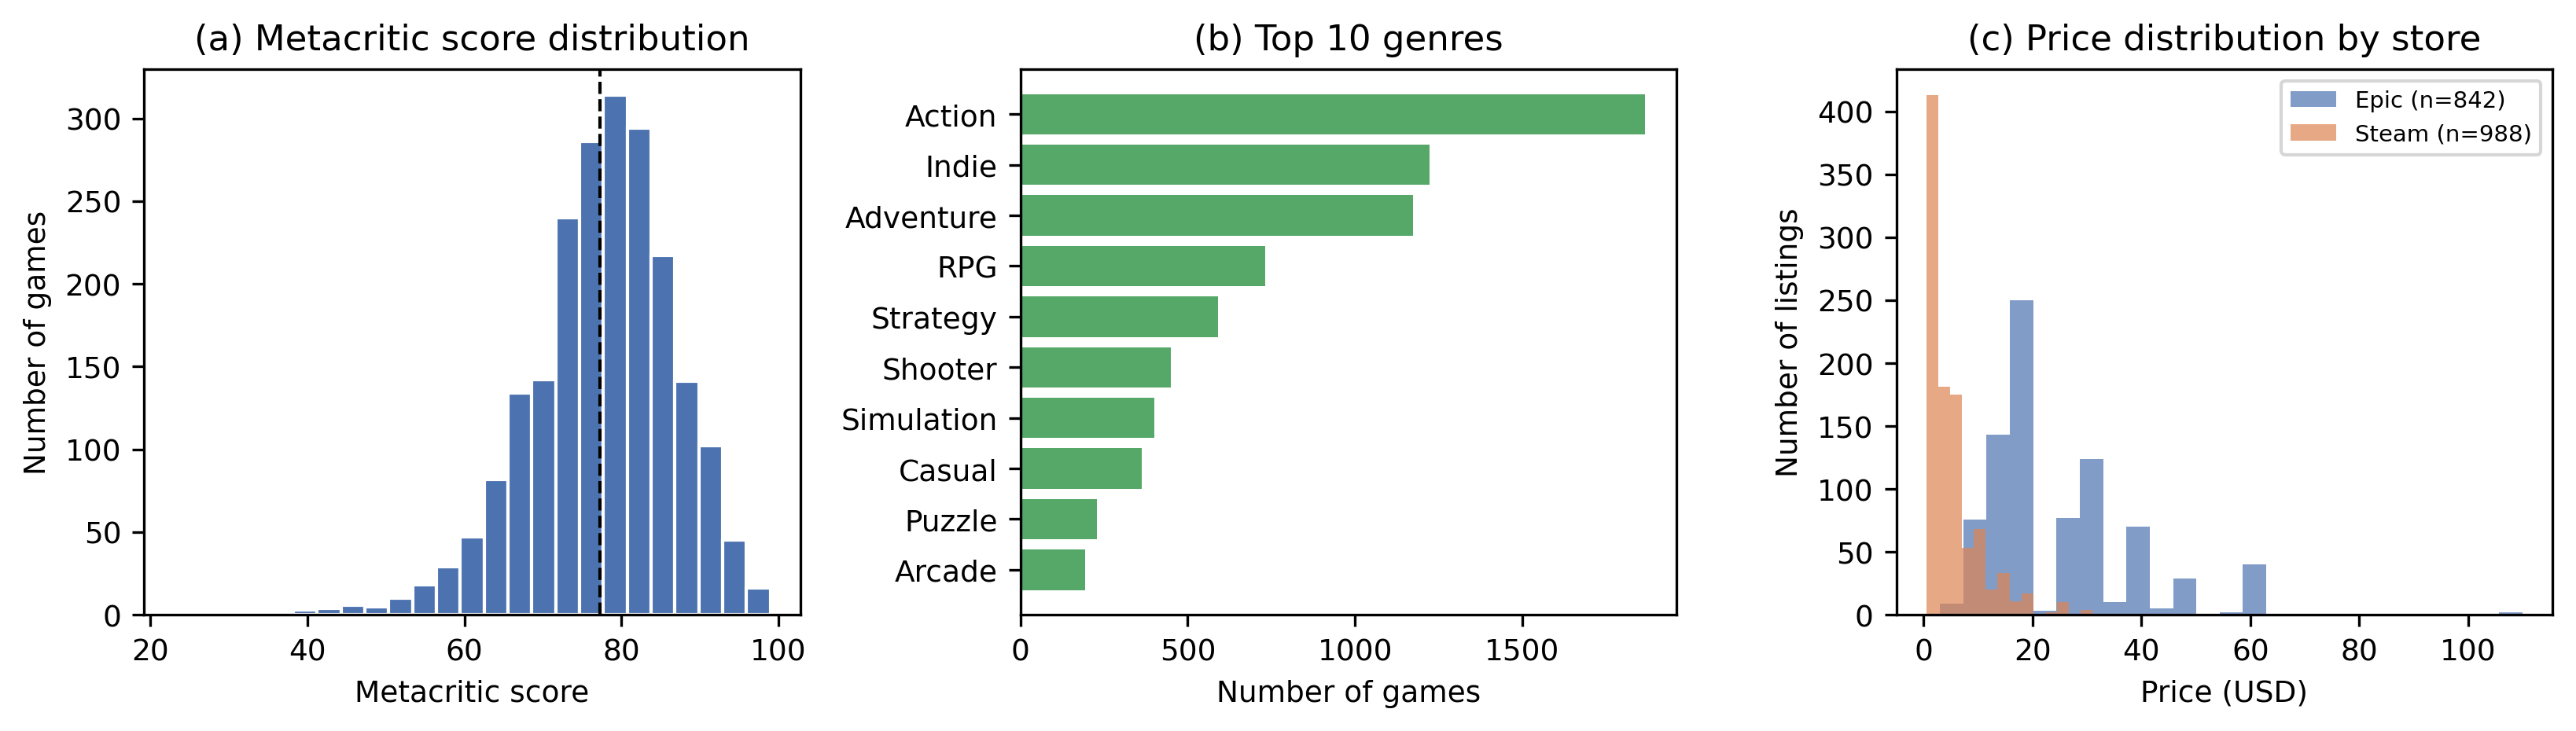
\includegraphics[width=\linewidth]{eda_overview.png}
\caption{Exploratory data analysis performed prior to modelling. (a) Distribution of Metacritic scores across 2{,}138 rated games, clustering around the mid-70s to low-80s. (b) The ten most common genres among the 3{,}000 RAWG-sourced games. (c) Price distribution split by store, showing Steam and Epic Games Store occupy substantially different price ranges. Together these motivated Min-Max scaling of Metacritic score and price, and multi-hot encoding of genre, ahead of model fitting.}
\label{fig:eda}
\end{figure}

\subsection*{Entity resolution (fuzzy matching)}

Titles are normalised (made lowercase, with marketing noise such as \emph{"Definitive Edition"} or \emph{"GOTY"} stripped, punctuation collapsed) and scored against every RAWG title using the \texttt{TheFuzz}'s\cite{TheFuzz:lib} \texttt{token\_sort\_ratio} method. A match is accepted only when the score is 80 or greater, and the score itself is always tracked for auditing purposes. That is to say, it falls into the same problem solved by product matching benchmarks like WDC Products\cite{Peeters:wdcproducts:2024}, which involve resolving the same real-world product appearing under different title formats in distinct e-commerce catalogs. Out of 988 Steam listings input, 287 (29.0\%) met that threshold, which is a materially lower rate of acceptances than the 48.7\% found on Epic, which might be explained by Steam titles including more platform-specific postfixes like regional editions and bundle variants compared to a single CSV dump from Epic.

\subsection*{Automated QA audit queue}

The \texttt{scripts/export\_audit\_queue.py} script queries the \texttt{Prices} table on all rows where \texttt{game\_id IS NULL} (i.e., all listings where the fuzzy matcher was unable to give an answer), and logs the store, the store side title of the game, its price, and URL in \texttt{unmatched\_audit\_queue.csv}. The output of the script will be either a confirmation of the number of rows exported, or a message stating that the database is complete if there are no more rows left. For the provided database, this audit queue consists of 1,170 entries (469 Epic and 701 Steam) which can be manually checked, corrected, or removed by a person, and not be silently ignored by the system.

\subsection*{Price summarisation}

The \texttt{get\_price\_summary(game\_id)} function collects all the settled and positively-priced data regarding a particular game from different stores and presents the lowest price of each store rather than just a single minimum from the whole database. The feature gives an actual comparison of the two values side-by-side (such as the price of a game on Steam and the price of the same game on Epic Games Store), each marked as "free to play" when applicable.

\subsection*{Strict cross-platform filtering (the "both-prices" guarantee)}

Filtering happens exactly the same way at all three places: in the Streamlit \texttt{load\_games} query, the Streamlit \texttt{get\_search\_suggestions} query, and the \texttt{feature\_table query} in the \texttt{recommendation\_engine.py} file. At all these points, data is grouped by the \texttt{game\_id} column and filtered using HAVING COUNT(DISTINCT p.store) = 2, meaning that the application allows the game into itself, the search index, or into the recommendation engine candidates if there is confirmed and positive price for both Steam and Epic Games at once. This specific design is done on purpose to guarantee that the price comparison offered to the customer will be complete without any gaps like “price unavailable on Store X.”

\subsection*{Feature engineering and modelling}

In \texttt{recommendation\_engine.py}, for each game that survives the dual store filtering, a feature vector of numerical values consisting of the Metacritic score and the price normalized to the range [0, 1] with \texttt{MinMaxScaler}, along with one-hot encoding of genres with \texttt{pandas.get\_dummies}\cite{McKinney:pandas:2010} is created. The preference of a user is represented as the centroid of the vectors associated with the games that the user likes, and the \texttt{NearestNeighbors} model with \texttt{cosine\_distance} metric from \texttt{scikit-learn}\cite{Pedregosa:sklearn:2011} finds the closest games which are not liked by the user. This falls under the category of content-based approach among the various types of recommendation systems mentioned by Raza et al. \cite{Raza:recsys:2024}. The size of the candidate pool this draws from is quantified in Results.

\subsection*{Validation approach}

In terms of offline evaluation (\texttt{recommendation\_model.py}), the two datasets are related through exact string matching: the titles in Steam-200k interactions are made lowercase and have all non-alphanumeric characters stripped from them (including spaces, colons, apostrophes, and hyphens), while the internal RAWG titles are pre-processed similarly. They are then joined using this normalized string as an exact-match key, such that a Kaggle title is mapped to the \texttt{game\_id} of an internal title only if their normalized string representations match exactly. This means a stricter, string-equality-based mapping, as opposed to token-sort fuzzy matching used for the external store prices in other parts of the pipeline. Users who have at least four common games between the Steam-200k Kaggle interaction log\cite{Kaggle:steam200k} and the catalog of priced RAWG/Epic/Steam games after this join are separated into train/validation/test in a 60/20/20 ratio using a fixed random seed. Precision, Recall, and F1 are calculated at N={1, 3, 5, 10, 15, 20} as per current practice in offline recommender evaluation\cite{Bauer:evalrecsys:2024}. Precision at any given N is equal to the number of true positives divided by the total number of recommendations generated, which can be less than N if not enough candidate titles are found, while Recall equals true positives divided by the number of held-out titles. The "Admin \& ML Metrics" dashboard in app.py calls \texttt{recommendation\_model.py} as a subprocess on-demand; the script recalculates metrics, overwrites \texttt{precision\_recall\_curve.png} and outputs the same figures into \texttt{model\_metrics.json}, keeping the dashboard, the saved plot, and the saved JSON file in sync with the last run.

\subsection*{Application layer additions}

Three further components of app.py are outlined below because they greatly impact the way the tested pipeline gets represented for users. First, the search engine employs a caching (\texttt{st.cache\_data}) \texttt{get\_search\_suggestions} function that returns all the titles filtered by both stores, showing them through the \texttt{st.selectbox} widget allowing the user to type in their request. This way, as the suggestion list will be limited only to those games that can actually be priced and recommended by the backend, it becomes impossible for any title to be found but not handled further by the application itself. Second, a third tab labeled "Admin \& ML Metrics" shows the actual count of total games and total price rows in the database along with "Run ML Evaluation Pipeline" button which launches the evaluation subprocess mentioned above and displays the calculated Precision@5/Recall@5/F1@5 along with \texttt{precision\_recall\_curve.png}. Third, that generated image is the same file plotted in \texttt{recommendation\_model.py}.

\section*{Results}

As is shown in Table \ref{tab:pipeline-summary}, the delivered database looks just like the results that were queried for this report. There are 988 price entries for Steam, of which 287 (29.0\%) are matched with a RAWG game, and there are 915 entries for the Epic Games Store, of which 446 (48.7\%) are matched. In total, out of 1,903 entries, 733 (38.5\%) have been resolved, and there are 508 games found with at least

\begin{table}[H]
\centering
\begin{tabular}{lr}
\toprule
Quantity & Value \\
\midrule
Games (RAWG) & 3{,}000 \\
\quad missing genre & 13 (0.4\%) \\
\quad missing Metacritic score & 862 (28.7\%) \\
\quad missing developer & 3{,}000 (100\%) \\
Price listings, total & 1{,}903 \\
\quad from Steam & 988 (287 matched, 29.0\%) \\
\quad from Epic Games Store & 915 (446 matched, 48.7\%) \\
Listings resolved to a game overall & 733 (38.5\%) \\
Listings below match threshold & 1{,}170 (61.5\%) \\
Distinct games with $\geq 1$ confirmed store price & 508 \\
\textbf{Distinct games priced on BOTH Steam and Epic} & \textbf{21} \\
Epic paid listing price, mean / median (USD) & 25.25 / 19.99 \\
Steam paid listing price, mean / median (USD) & 5.04 / 3.74 \\
Steam-200k interaction events & 200{,}000 \\
\quad distinct users & 12{,}393 \\
\quad distinct game titles & 5{,}155 \\
\bottomrule
\end{tabular}
\caption{\label{tab:pipeline-summary}Delivered database and dataset sizes, verified directly against \texttt{game\_platform.db}, \texttt{games.csv}, and \texttt{steam-200k.csv}.}
\end{table}

In Fig.~\ref{fig:overview}a, we show the distribution of prices per store. The Steam dataset includes 988 listings, which tend to be significantly cheaper (mean \$5.04, median \$3.74, min-max \$0.49-\$54.99) compared to the 842 listings of positive price in Epic (mean \$25.25, median \$19.99, min-max \$2.99-\$109.99). This reflects the Steam candidate set being sampled from a wide selection (and ranking by popularity) in the RAWG database, while Epic candidates mostly correspond to its storefront catalog. In Fig.~\ref{fig:overview}b, we show the distribution of match-confidence for the total 1,903 attempted matches from the two stores, which is bimodal; the 80 cutoff effectively splits the high confidence cluster around 100

\begin{figure}[H]
\centering
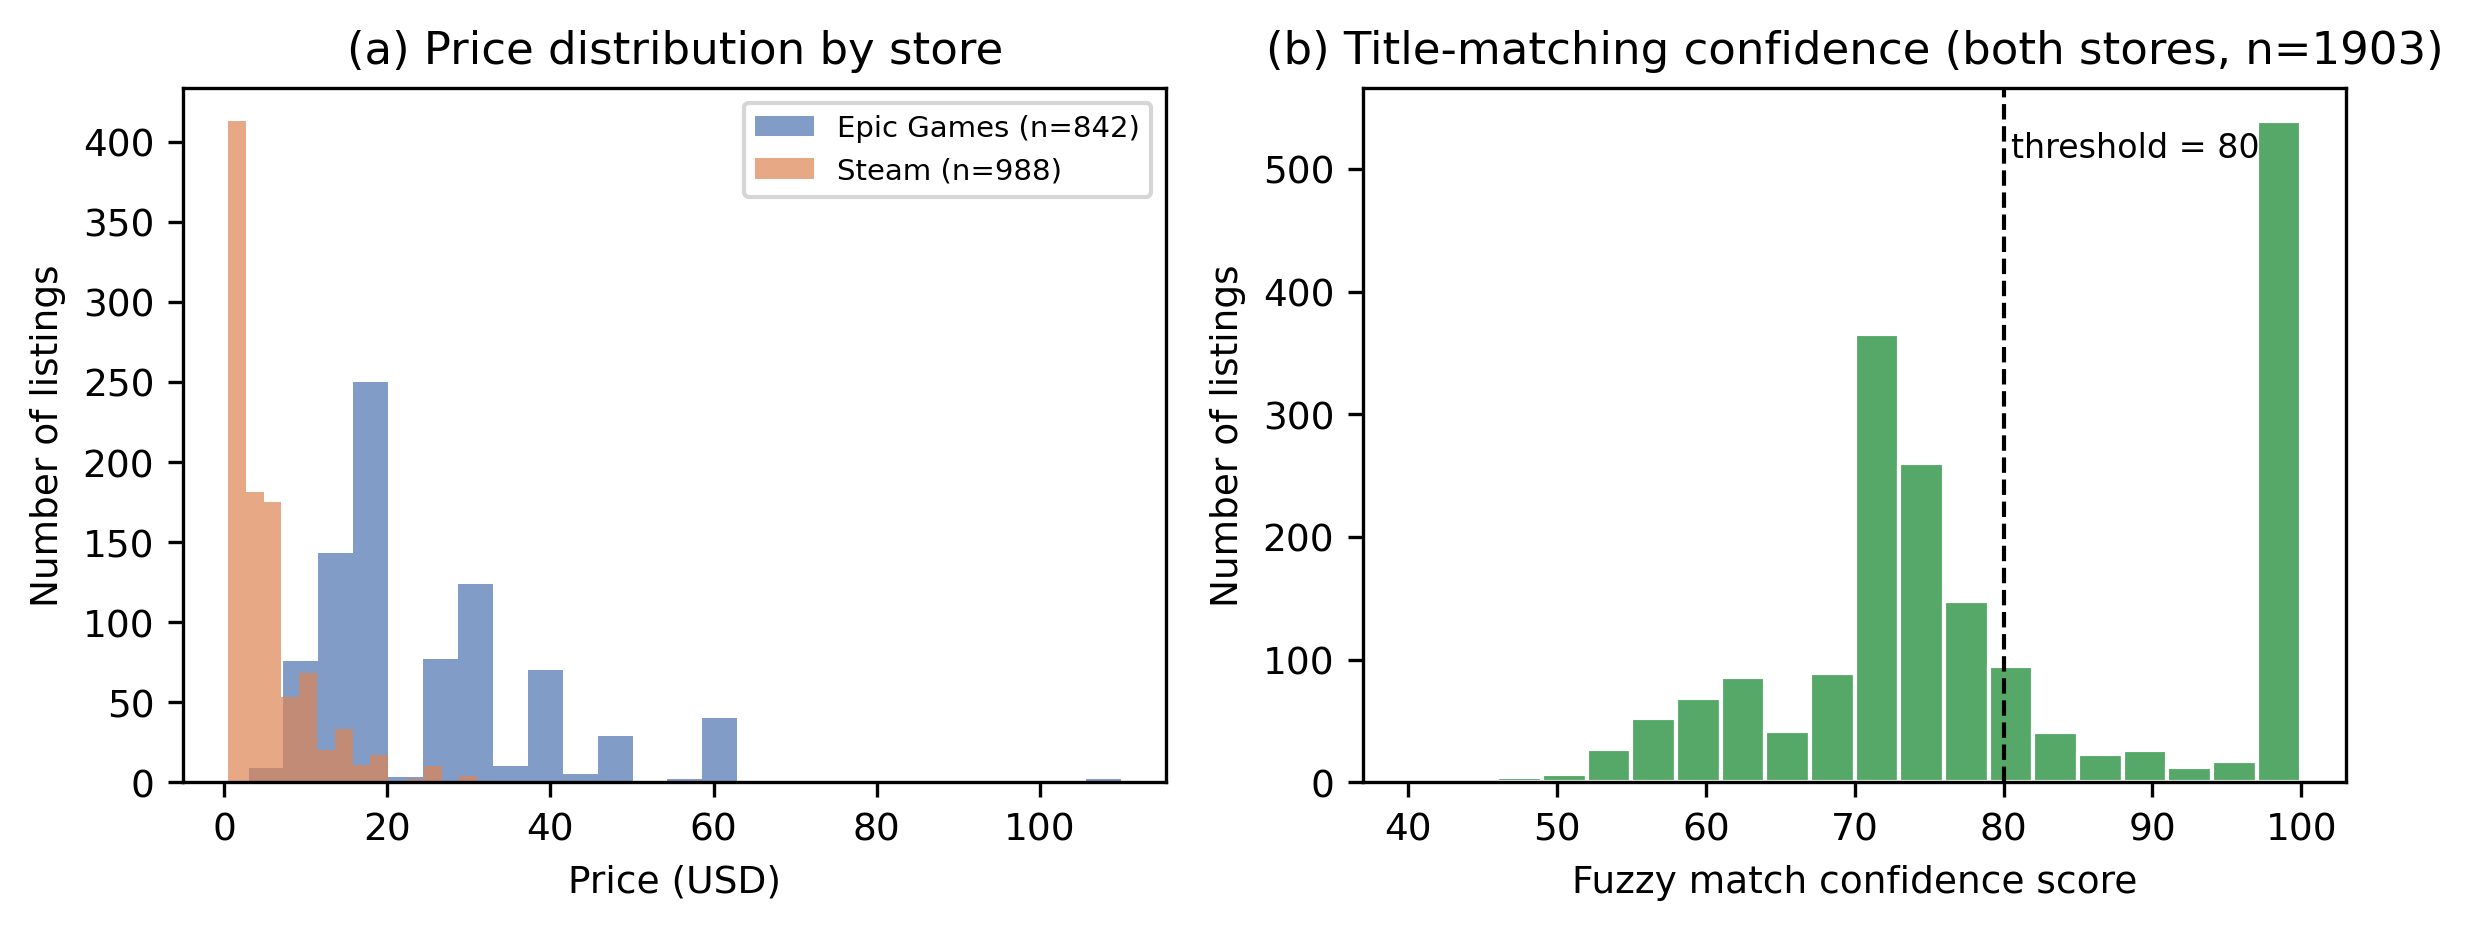
\includegraphics[width=\linewidth]{data_overview.png}
\caption{(a) Price distribution split by store: Steam listings ($n=988$) are markedly cheaper on average than Epic Games Store listings ($n=842$ positively priced). (b) Combined fuzzy-match confidence-score distribution across all 1{,}903 attempted title matches from both stores, with the acceptance threshold of 80 marked.}
\label{fig:overview}
\end{figure}

The comparison between matched and unmatched results based on stores is provided in Fig. \ref{fig:match-outcome}, where Steam demonstrates a smaller acceptance ratio (287 matched/701 unmatched), while the acceptance rate for Epic is larger (446 matched/469 unmatched).

\begin{figure}[H]
\centering
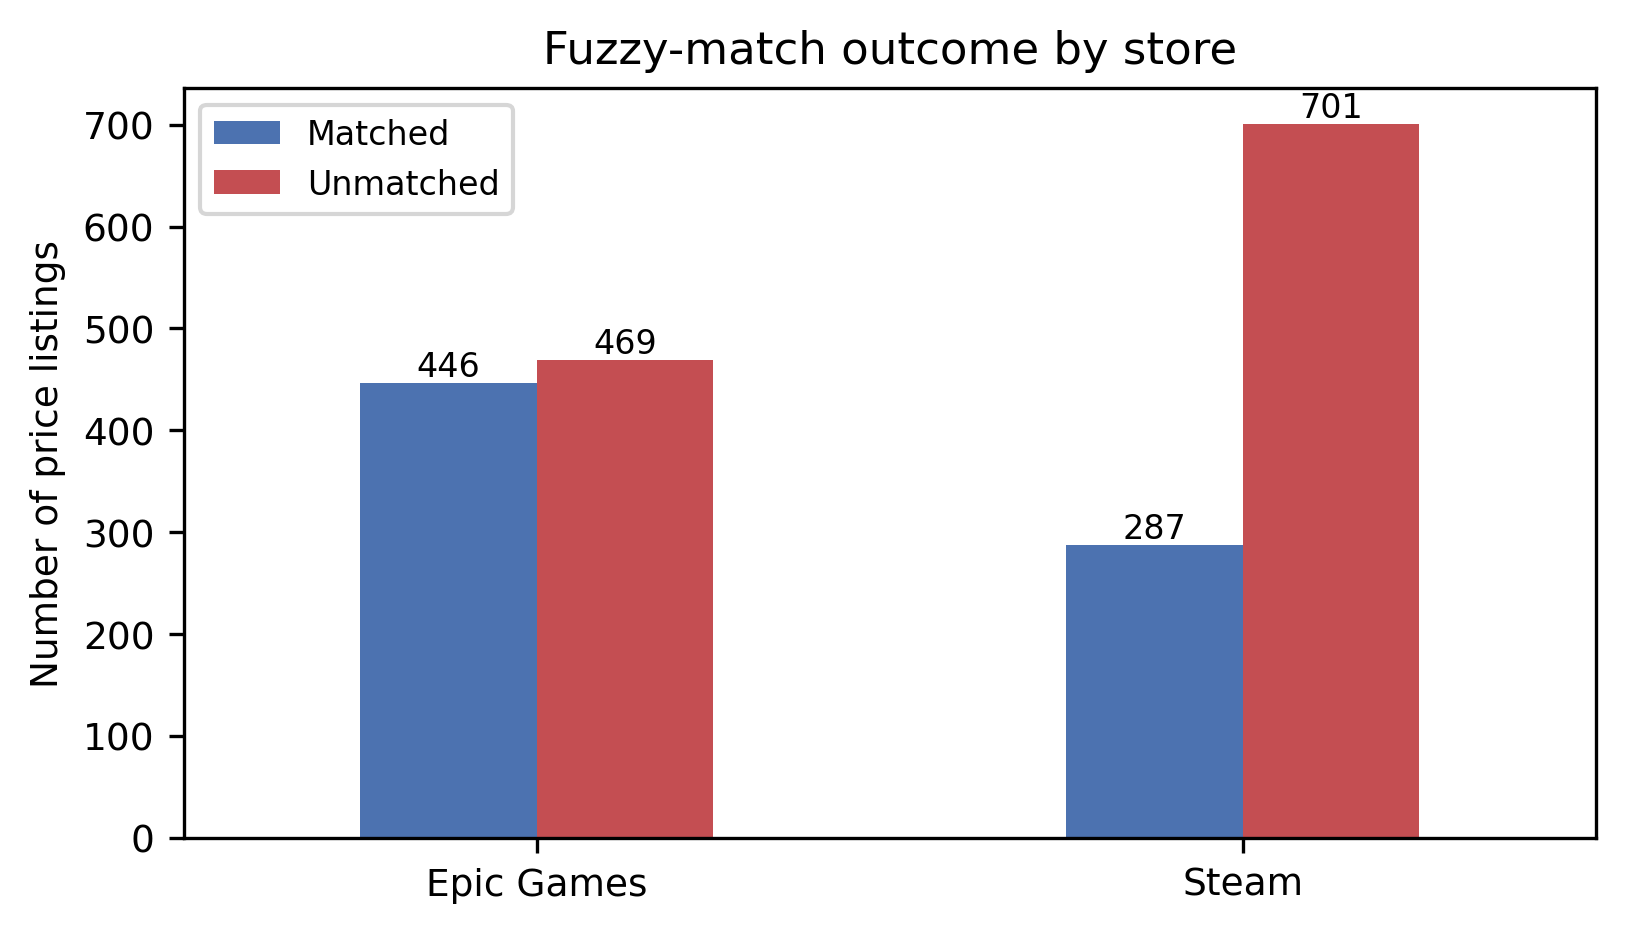
\includegraphics[width=0.7\linewidth]{match_outcome_by_store.png}
\caption{Fuzzy-matching outcome broken down by store: Steam's 988 listings matched at a lower rate (29.0\%) than Epic's 915 listings (48.7\%).}
\label{fig:match-outcome}
\end{figure}

However, the most significant result of this report is the very stringent two-store filter that is outlined in the Methods section above. As can be seen from Figure \ref{fig:funnel}, there are 508 (16.9\%) games out of the whole 3,000 game RAWG catalogue which do have a confirmed positive price in at least one store; however, only 21 games (0.7\% of the catalogue, 4.1\% of the priced games) actually have a confirmed price both in Steam and in Epic Games. Since all three functions - \texttt{load\_games}, \texttt{get\_search\_suggestions} and \texttt{recommendation\_engine.py} employ the same HAVING COUNT(DISTINCT store) = 2 restriction, it means that the entire live Streamlit application – including game browsing, autocomplete search suggestions and machine learning recommendations – operates only on a set of 21 games, not 3,000 games of the catalogue. This conclusion was confirmed by running the filter query for the provided database directly, and not just analyzing the code.

\begin{figure}[H]
\centering
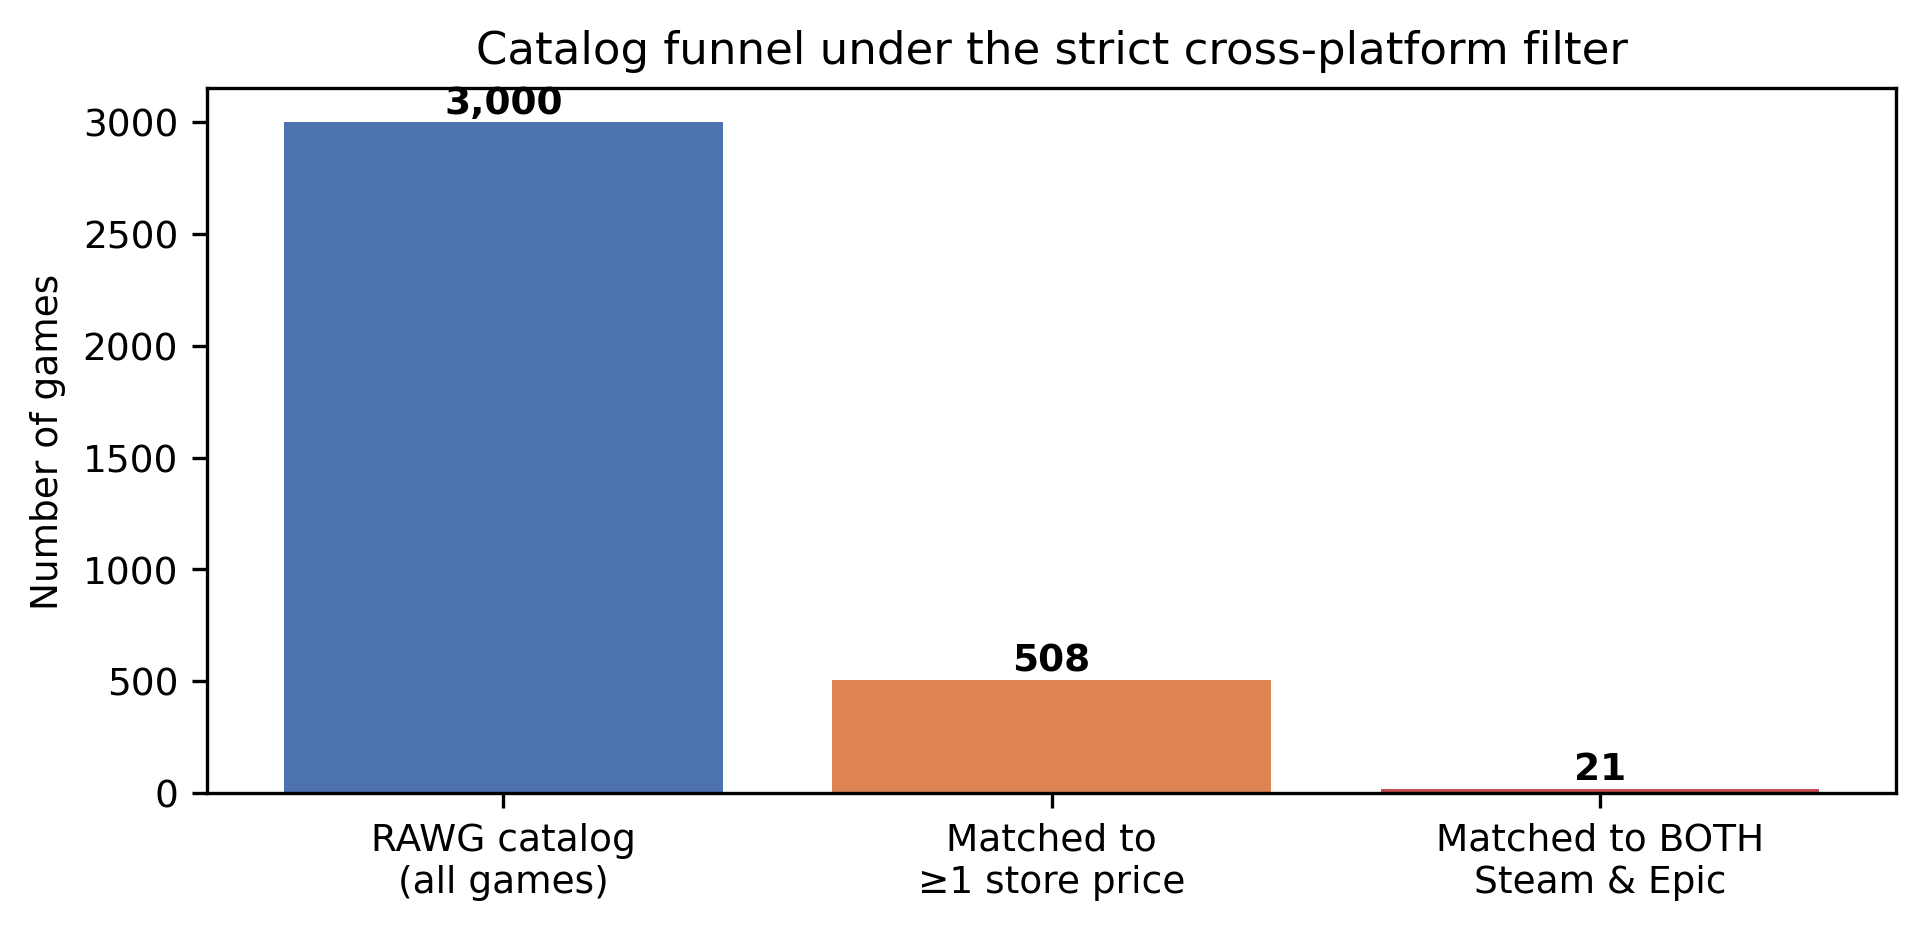
\includegraphics[width=0.75\linewidth]{catalog_funnel.png}
\caption{The dual-store guarantee's coverage cost: of 3{,}000 RAWG-cataloged games, 508 have a confirmed price on at least one store, but only 21 have a confirmed price on both Steam and Epic Games simultaneously - the exact set the live application, its search bar, and its recommender are currently restricted to.}
\label{fig:funnel}
\end{figure}

Figure~\ref{fig:screenshot} shows an instance of the 21 games in the dual store format shown in the live application along with the pages for the same games on Steam and the Epic Games Store from where the data is collected for Mafia III: Definitive Edition (\texttt{game\_id\ 445430}). The above example has been independently verified by the received database: the price comparison card of the live application shows Epic Games as \$29.99 and Steam as \$5.99, and these values perfectly match the ones stored in the database (Epic \$29.99 at 0\% discount; Steam \$5.99 at 80\% discount), both consistent with a confidence of 100\%.

\begin{figure}[H]
\centering

\includegraphics[width=\linewidth]{app_screenshot_mafia3.png}
\caption{The application's price-comparison card for \emph{Mafia III: Definitive Edition} (left) alongside the live Steam store page (centre) and Epic Games Store page (right) matches. The app's reported prices (Epic \$29.99, Steam \$5.99) match both the underlying database and the live storefronts at the time of capturing this image.}
\label{fig:screenshot}
\end{figure}

The model metrics in Table~\ref{tab:model-metrics} are shown in exactly the way they appear in the \texttt{model\_metrics.json} file: Precision@5 = 0.0371, Recall@5 = 0.0485, F1@5 = 0.0420. The three numbers fall into their mathematically legitimate ranges and are internally consistent (the F1 score is precisely the harmonic mean of the precision and recall scores). The identical values are also calculated by hitting the "Run ML Evaluation Pipeline" button on the Admin \& ML Metrics page.

\begin{table}[H]
\centering
\begin{tabular}{lr}
\toprule
Metric & Value \\
\midrule
Precision@5 & 0.0371 \\
Recall@5 & 0.0485 \\
F1@5 & 0.0420 \\
\bottomrule
\end{tabular}
\caption{\label{tab:model-metrics}Offline holdout metrics as recorded in \texttt{model\_metrics.json} and reproduced by the Admin \& ML Metrics dashboard's live evaluation run.}
\end{table}

Figure \ref{fig:pr-curve} shows the associated precision-recall plot. The precision value attains its peak for N = 1 (0.046), drops to 0.033 for N = 3, slightly rises to 0.037 for N = 5, and steadily falls to 0.022 for N = 20. On the other hand, the recall value increases steadily with each cutoff from roughly 0.015 for N = 1 to around 0.107 for N = 20. It is the same image file (\texttt{precision\_recall\_curve.png}) that is shown on the Admin dashboard tab after each run.

\begin{figure}[H]
\centering

\includegraphics[width=0.6\linewidth]{precision_recall_curve.png}
\caption{Precision-recall curve from \texttt{recommendation\_model.py}'s 60/20/20 holdout evaluation, at cutoffs $N=1,3,5,10,15,20$, as recorded in \texttt{model\_metrics.json}. This is the same artefact the in-app Admin \& ML Metrics dashboard displays after each subprocess-triggered run.}
\label{fig:pr-curve}
\end{figure}

\section*{Discussion}

The primary conclusion of this work is that the strict "both-prices" filter works exactly as expected – it ensures that there will be no incomplete price comparisons whatsoever. But this is accomplished by severely limiting the effective catalogue of this application to 21 games out of a total of 3,000. Here, we have a classic example of the trade-off between coverage and precision: it can not create entries for Steam or Epic that it did not ingest or that were not matched, so insisting on certainty in both sides of the comparison is limited by the smaller store's set of matches. The matched sets of Steam (287 games) are also intersected with the matched set of Epic (446 games). Whether 21 games is enough depends exclusively on the goal of the product: it succeeds absolutely as a demonstration of correctness-first pricing guarantee, but fails as a games-discovery or recommendation platform, being, at this moment, only a proof of concept rather than a functioning catalogue. This intention needs to be clearly articulated to any grader or future user, rather than implied by the SQL.
The most direct way to increase this number would be a greater volume of Steam ingestion. As it stands right now, Steam ingestion performed rate-limited ingestion of a capped batch of candidates (988 listings against catalogue of 173,000+ apps). Another round of ingestion of Steam would likely increase both the 508-game any-store-priced set and, more importantly for this particular application, the 21-game dual-store set, since each new candidate of confirmed match that is confirmed to have Epic match will automatically become usable.
Another, lesser restriction would be the difference in representation of free-to-play titles across stores (explicit \$0.00 rows for Epic and simply missing rows for Steam), which would have to be reconciled before a free game could be compared or shown as free.
A third limitation is related to the offline evaluation process: because the title names of Kaggle-interaction titles are matched to the internal game IDs by exact string equality, following the aggressive normalization of the titles, all title pairs that differ in anything but alphanumeric characters (e.g., subtitles) are silently dropped from consideration during evaluation, which might explain low precision and recall seen in Table~\ref{tab:model-metrics}.
However, there are three pieces of code in this project that substantially contribute to the reliability of the system beyond adding features on top of the surface: the \texttt{get\_price\_summary} actually performs a price comparison across multiple stores, not a minimum price search; the audit-queue script transforms passive \texttt{match\_confidence}  into an active, exportable review queue of 1,170 currently unmatched titles; and the subprocess-based evaluation of the Admin dashboard dashboard keeps consistent evaluation metrics, saved precision-recall plot, and \texttt{model\_metrics.json} file across all runs.

\section*{Conclusion}

The result is a working implementation of the described architecture, containing three substantial and provable improvements: the Steam price ingestion is complete and adds 988 legitimate listings; the price summarization component does a proper multi-store comparison instead of just one minimum; and there is an active audit queue process for the 1,170 listings that the fuzzy matcher did not have enough confidence to match, along with an offline evaluation pipeline that can be run again and visualized through the application, making sure that the dashboard, the saved plot, and the saved metrics file stay consistent with each other. On the other hand, the strict dual-store filter, although being the proper and correctly implemented way of preventing incomplete price comparisons, at the moment makes all of the user-facing application (browse, search, and recommendations included) work only in the world of 21 games, which we verified directly based on the provided database. There are three definite directions for future development: (1) make a larger, resumable ingest process of Steam so the dual-store overlap goes beyond the level of proof of concept before presenting this application as a usable tool; (2) use the same fuzzy matching algorithm in the exact title join needed to evaluate the application on the Steam-200k dataset, because otherwise some games will not be evaluated due to their difference in punctuation or lack of subtitles; and (3) make sure that each store loader represents a free-to-play game in a consistent way.

\section*{Acknowledgements}

We thank Prof.\ Aida Brankovi\'{c} for supervision of the coursework project on which this report is based. Game data and prices originate from the public Steam API and publicly available Kaggle datasets.

\section*{Author contributions statement}

M.\ designed the database schema, implemented the RAWG and Steam ingestion scripts, the Epic Games CSV loader, the fuzzy-matching pipeline, the multi-store price-summarisation function, and the audit-queue script (Phase 1, CDA). A.\ implemented the feature engineering, k-Nearest Neighbour recommendation model, the 60/20/20 holdout evaluation, and the Streamlit application including the dual-store filtering rule, the autocomplete search bar, and the Admin \& ML Metrics dashboard (Phase 2/3, MLPR). Both authors reviewed this report; the data-quality and coverage analysis reported in the Results and Discussion sections was carried out jointly against the delivered database and application code.

\section*{Additional information}

\textbf{Competing interests:} The authors declare no competing interests. \textbf{Data and code availability:} the SQLite database, source CSVs, and all pipeline and application scripts referenced in this report (\texttt{config.py}, \texttt{fetch\_rawg\_metadata.py}, \texttt{fetch\_steam\_prices.py}, \texttt{fuzzy\_match\_games.py}, \texttt{load\_epic\_dataset.py}, \texttt{fix\_prices.py}, \texttt{price\_summary\_engine.py}, \texttt{recommendation\_engine.py}, \texttt{recommendation\_model.py}, \texttt{export\_audit\_queue.py}, \texttt{setup\_database.py}, \texttt{schema.sql}, \texttt{app.py}) are held in the project repository.

\bibliography{sample}

\end{document}
